\section{Performance Evaluation}
\subsection{Efficacy of the ODE model}
\label{subsec:pe_valid}
\begin{figure}
  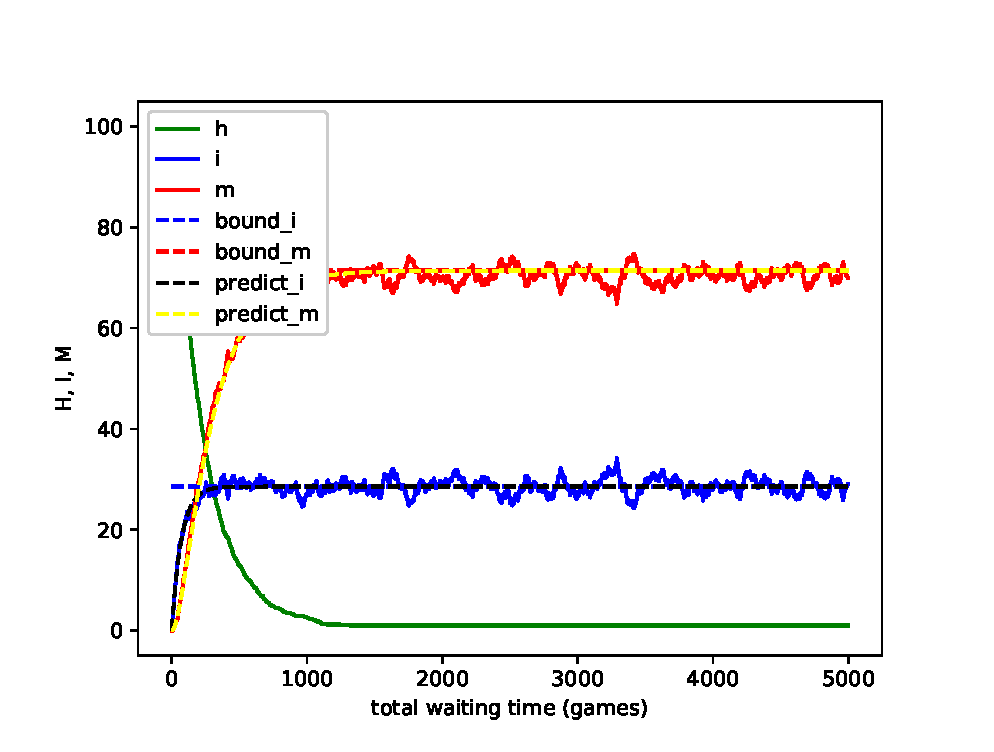
\includegraphics[width=.45\textwidth]{fig/twohop_predict_sim.eps}
  \caption{$I(t)$ and $M(t)$ with time $t$ obtained from prediction and simulations
  when $\beta = 0.004$, $\rho = 0.01$ and $N=100$. Here $h$ and $i$ is the mean value of $20$ simulations.}
  \label{fig:twohop_predict_wod}
\end{figure}
Fig.~\ref{fig:twohop_predict_wod} shows that the change of the states
in the experiments conforms to
the solved solutions.

\subsection{Optimal solution of selfish detection}
\begin{figure}
  \centering
  {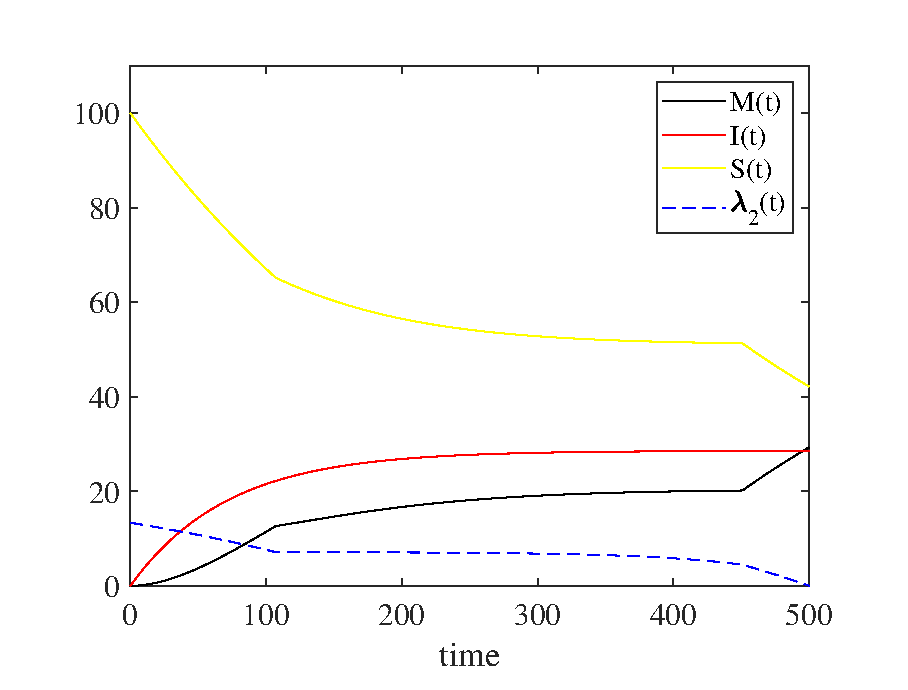
\includegraphics[width=0.47\textwidth]{fig/state.eps}}
     \caption{State variable of analysis with time.}
     \label{fig:pe_opt_state_time}
\end{figure}
\begin{figure}
  \centering
  {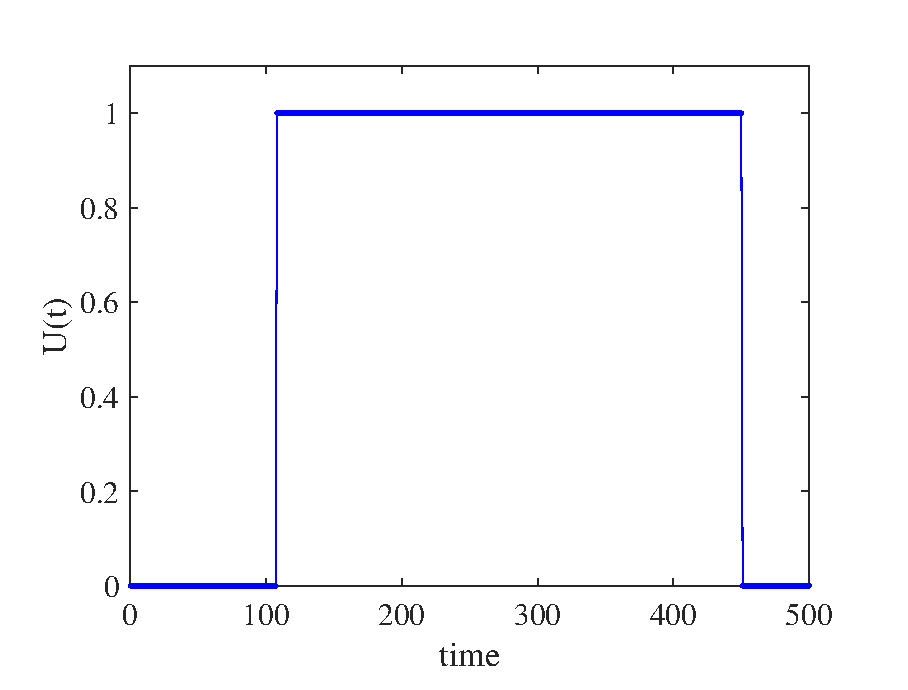
\includegraphics[width=0.47\textwidth]{fig/Ut.eps}}
     \caption{Control variable of analysis with time.}
     \label{fig:pe_opt_control_Ut}
\end{figure}
\begin{figure}
  \centering
  {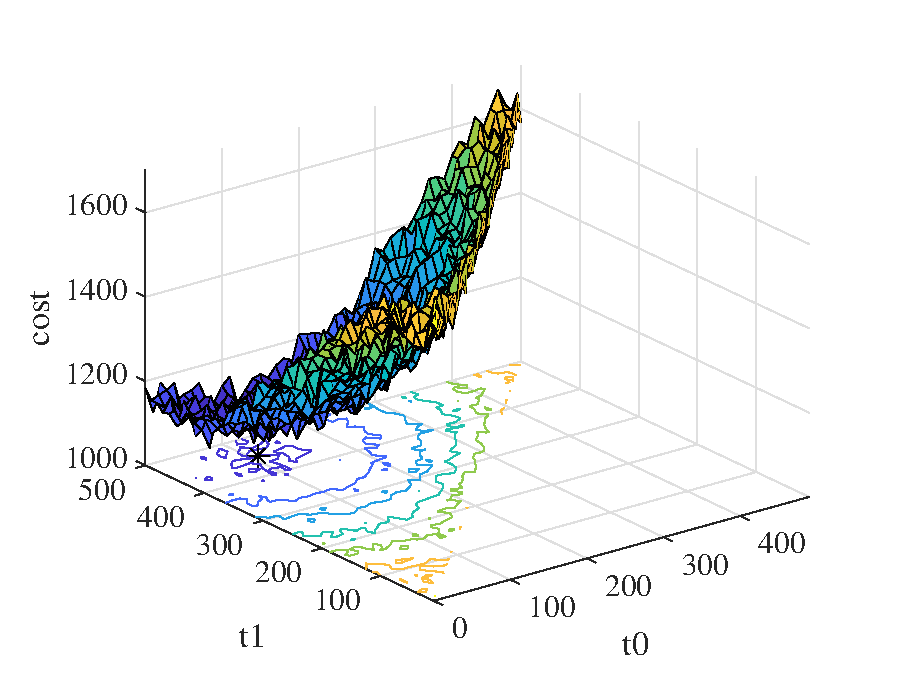
\includegraphics[width=0.47\textwidth]{fig/cost_all_t0t1.eps}}
     \caption{Different choices of $t0$ and $t1$.}
     \label{fig:pe_diff_choices}
\end{figure}
